\documentclass[12pt, titlepage]{article}

\usepackage{booktabs}
\usepackage{tabularx}
\usepackage{hyperref}
\hypersetup{
    colorlinks,
    citecolor=black,
    filecolor=black,
    linkcolor=red,
    urlcolor=blue
}
\usepackage[round]{natbib}
\usepackage{fullpage}
\usepackage{scrextend}
\usepackage{amsmath}
\usepackage{graphicx}
\graphicspath{ {image/} }

%%%%  lines 19-61 from https://tex.stackexchange.com/questions/83882/how-to-highlight-python-syntax-in-latex-listings-lstinputlistings-command
%\usepackage[utf8]{inputenc}

% Default fixed font does not support bold face
\DeclareFixedFont{\ttb}{T1}{txtt}{bx}{n}{12} % for bold
\DeclareFixedFont{\ttm}{T1}{txtt}{m}{n}{12}  % for normal

% Custom colors
\usepackage{color}
\definecolor{deepblue}{rgb}{0,0,0.5}
\definecolor{deepred}{rgb}{0.6,0,0}
\definecolor{deepgreen}{rgb}{0,0.5,0}

\usepackage{listings}

% Python style for highlighting
\newcommand\pythonstyle{\lstset{
language=Python,
basicstyle=\ttm,
otherkeywords={self},             % Add keywords here
keywordstyle=\small\ttb\color{deepblue},
emph={MyClass,__init__},          % Custom highlighting
emphstyle=\small\ttb\color{deepred},    % Custom highlighting style
stringstyle=\small\color{deepgreen},
frame=,                         % Any extra options here
showstringspaces=false            % 
}}


% Python environment
\lstnewenvironment{python}[1][]
{
\pythonstyle
\lstset{#1}
}
{}

% Python for external files
\newcommand\pythonexternal[2][]{{
\pythonstyle
\lstinputlisting[#1]{#2}}}

% Python for inline
\newcommand\pythoninline[1]{{\pythonstyle\lstinline!#1!}}

\newcommand{\progname}{SpecGen}

\newcounter{testnum} %Instance Number
\newcommand{\tthetestnum}{T\thetestnum}
\newcommand{\testref}[1]{T\ref{#1}}
\newcommand{\sref}[1]{\S~\ref{#1}}

%% Comments

\usepackage{color}

\newif\ifcomments\commentstrue

\ifcomments
\newcommand{\authornote}[3]{\textcolor{#1}{[#3 ---#2]}}
\newcommand{\todo}[1]{\textcolor{red}{[TODO: #1]}}
\else
\newcommand{\authornote}[3]{}
\newcommand{\todo}[1]{}
\fi

\newcommand{\wss}[1]{\authornote{blue}{SS}{#1}}
\renewcommand{\sp}[1]{\authornote{magenta}{SP}{#1}}


\begin{document}
\pagenumbering{gobble}

\title{CAS 741: Test Plan\\[10pt]\Large Aqueous Speciation Diagram Generator}
\author{Steven Palmer\\\texttt{palmes4}}
\date{\today}
	
\maketitle

\pagenumbering{roman}

\setcounter{secnumdepth}{0}

\section{Revision History}

\begin{table}[hp]
\caption{Revision History} \label{TblRevisionHistory}
\begin{tabularx}{\textwidth}{llX}
\toprule
\textbf{Date} & \textbf{Developer(s)} & \textbf{Change}\\
\midrule
10.13.2017 & S. Palmer & First revision of document\\
10.25.2017 & S. Palmer & Revision 0 submission\\
12.18.2017 & S. Palmer & Revision 1\\
\bottomrule
\end{tabularx}
\end{table}

~\newpage


\section{Symbols, Abbreviations and Acronyms}

\renewcommand{\arraystretch}{1.2}
\begin{tabular}{l l} 
  \toprule		
  \textbf{symbol} & \textbf{description}\\
  \midrule
  \progname{} & The Aqueous Speciation Diagram Generator program\\  
  SRS & Software Requirements Specification\\
  T & Test\\
  \bottomrule
\end{tabular}\\

\newpage

\tableofcontents


\newpage


\pagenumbering{arabic}

\setcounter{secnumdepth}{3}

\section{General Information}

This document provides a detailed description of the testing that will be 
carried out on the Aqueous Speciation Diagram Generator program (herein referred 
to as \progname{}).  Complementary documents include the 
System Requirement Specifications, Module Guide and Module Interface Specification.  
The full documentation and 
implementation can be found \href{https://github.com/palmerst/cas741_sp}{here}.

\subsection{Purpose}
The purpose of this document is to provide a comprehensive plan for testing the 
\progname{} software against the requirements described in the
\progname{} SRS.  \wss{An explicit web-link to your GitHub repo would be nice.}

\subsection{Scope}
The test plan is narrowed to the following scope:
\begin{itemize}
\item The tests outlined in this document are limited to the verification of the 
  requirements given in the \progname{} SRS.  The validation of the requirements 
  will be carried out via correspondence with Dr.\ Scott Smith 
  (Wilfrid Laurier University).
  \wss{Add information on Dr.\ Smith's affiliation}
\item The tests outlined in this document are limited to dynamic tests only.  
  Due to the small size and low complexity of the \progname{} program, no formal
  static testing (code walkthroughs, code inspections, etc.) will be carried out.
\item The \progname{} software will be written in Python.  The testing of 
  implementations in other languages will not be considered in this document.
\end{itemize}

\section{Plan}
\label{SecPlan}
	
\subsection{Software Description}
Chemical speciation refers to the stable (equilibrium) distribution of chemical 
species in a given chemical system.   Speciation diagrams, which plot species 
concentrations against an independently varied parameter of the system, are 
useful tools for displaying speciation data in a concise and easy to use format.  

\progname{} will produce a speciation diagram given a set of chemical reactions, 
equilibrium constants, and element totals that define a chemical system.  
\progname{} will be specific to speciation of ions in aqueous systems under 
varying pH, which is of particular importance in the fields of aqueous process 
engineering and hydrometallurgy.  The diagram generated by \progname{} will plot 
speciation of all aqueous species (excluding H$^+$ and OH$^-$) across the pH 
range 0 to 14.

\subsection{Test Team}
The test team includes the following members:
\begin{itemize}
\item Steven Palmer
\end{itemize}

\subsection{Automated Testing Approach}
The automated testing for \progname{} will be carried out using a set of unit 
and integration tests.  A test coverage analysis of these tests will be 
carried out to ensure that testing is as complete as possible.  The target 
for this analysis is 100\% statement coverage. 

Regression testing will be used during the implementation stage and for any 
future changes.  Since \progname{} is small in scope and will be implemented 
by a single developer, other forms of automated testing, such as continuous 
integration testing, will not be considered.


\subsection{Verification Tools}
The following tools will be used to facilitate testing:

\begin{enumerate}
\item {\bf PyTest} (a unit testing framework for Python) will be used to write 
  and run unit tests
\item {\bf Coverage.py} will be used to assess test coverage
\item {\bf make} will be used to automate the building and execution of the test 
  program
\end{enumerate}



\subsection{Non-Testing Based Verification}
N/A

\section{System Test Description}

\subsection{Tests for Functional Requirements}

\noindent {\bf T\refstepcounter{testnum}\thetestnum \label{T_DiagFe}: Diagram generation of FeOH$_3$ system}\\
\begin{addmargin}[2em]{0em}
\begin{description}
\item[Type:] Functional, Automatic, Integration
					
\item[Initial State:] ~\newline

\begin{python}
feSys = ChemSys()
feSys.registerRxn(
  "(Fe)3+ + (H2O)l = (Fe(OH))2+ + (H)+ , -2.19"
)
feSys.registerRxn(
  "(Fe)3+ + 2(H2O)l = (Fe(OH)2)+ + 2(H)+ , -5.67"
)
feSys.registerRxn(
  "(Fe)3+ + 4(H2O)l = (Fe(OH)4)- + 4(H)+ , -21.6"
)
feSys.registerTotal(
  "Fe", 0.000010
)
\end{python}
					
\item[Input:] ~\newline

\begin{python}
feSys.specGen("fe")
\end{python}

					
\item[Output:] ~\newline

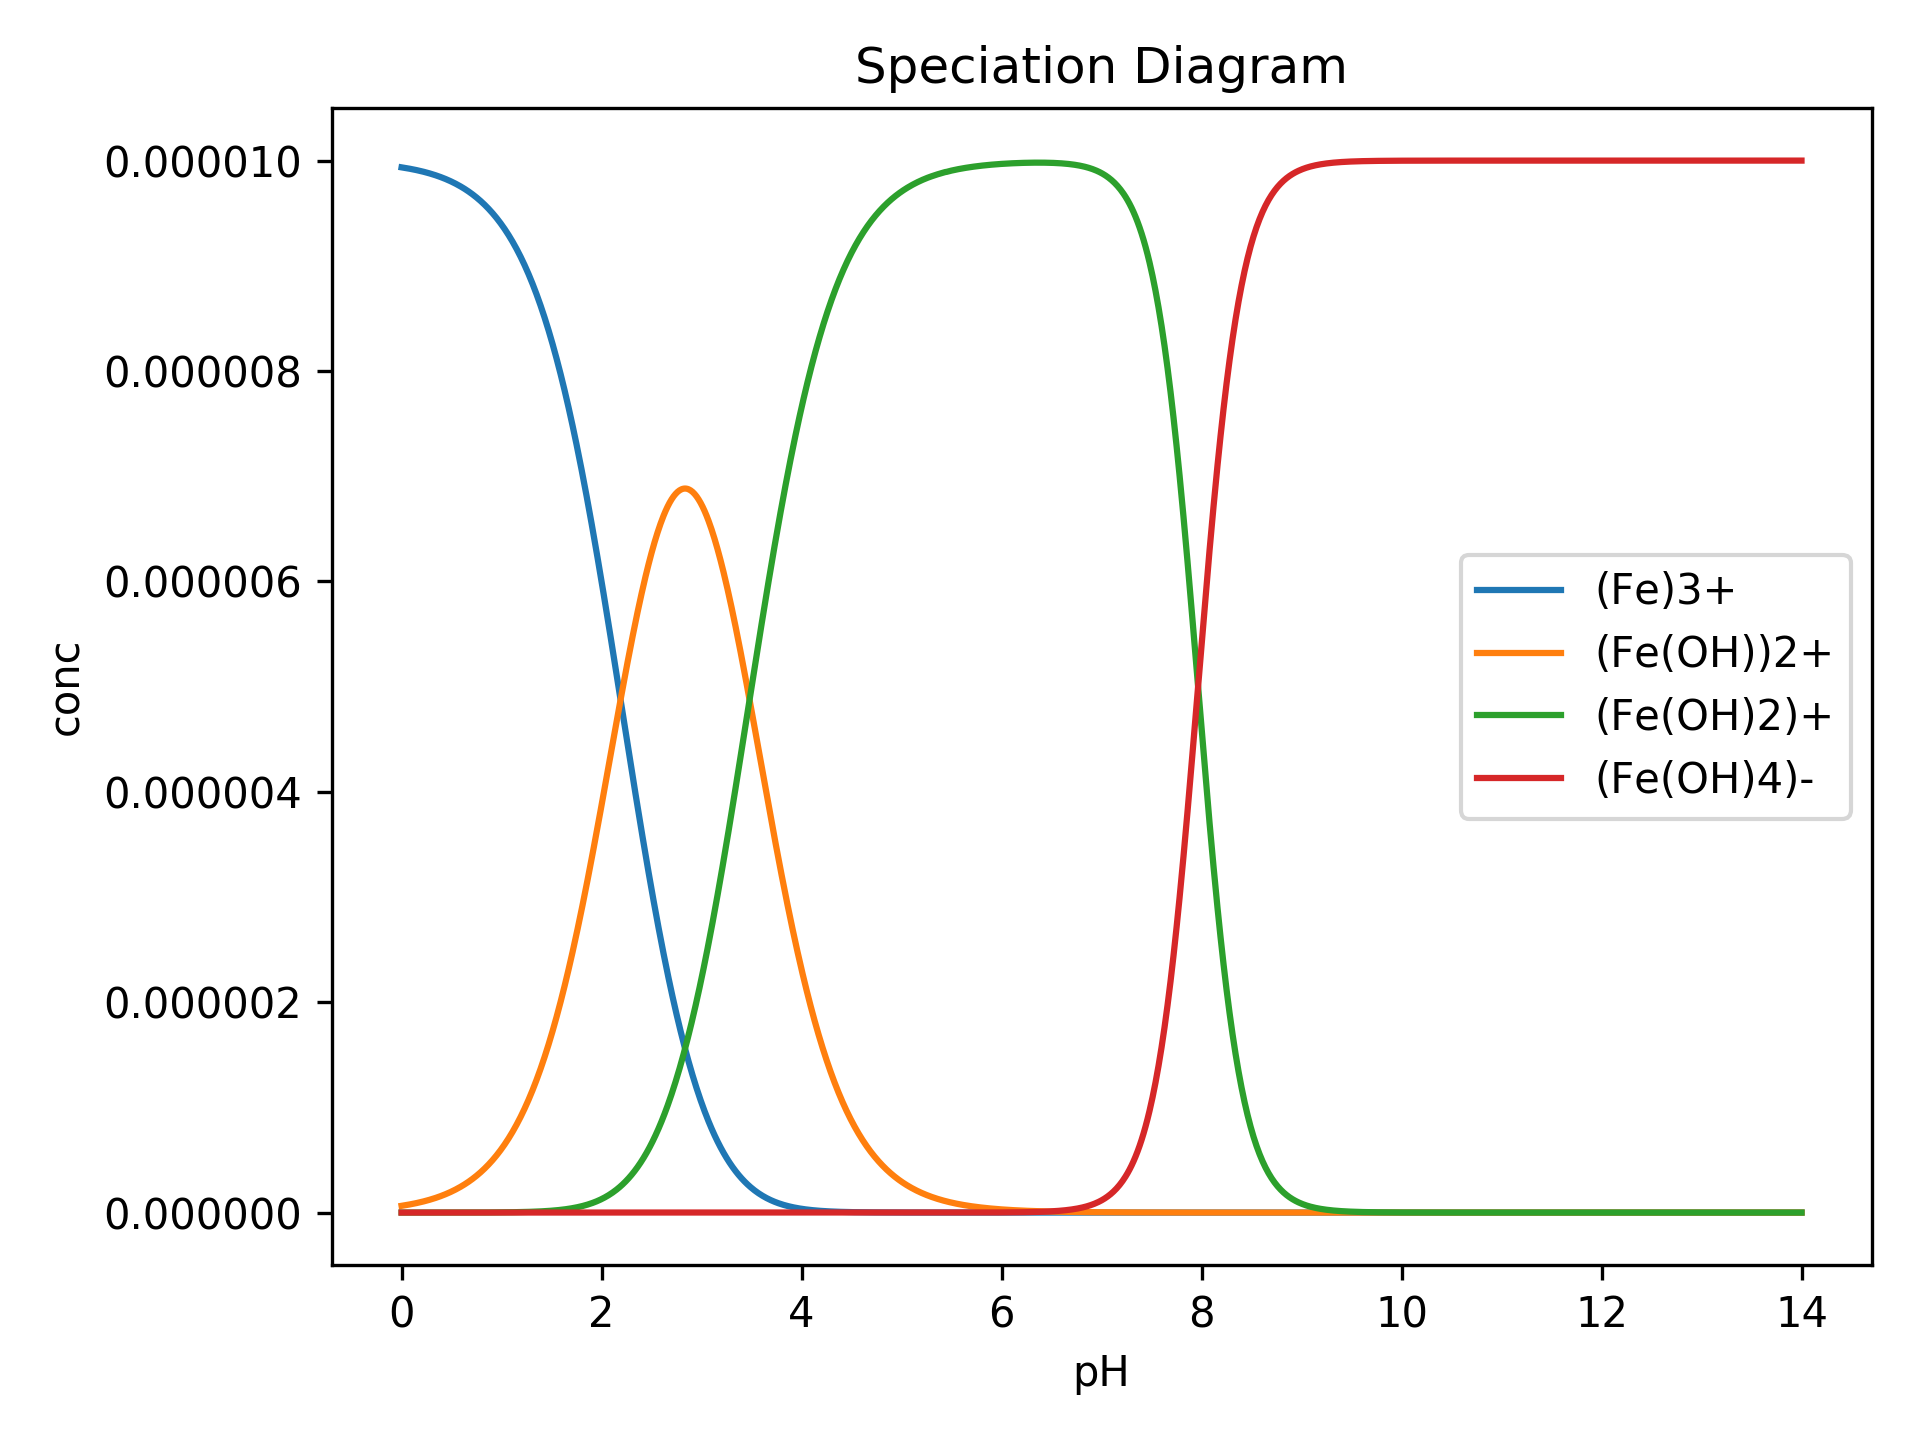
\includegraphics[width=0.7\textwidth]{fe_syst}

					
\item[How test will be performed:] Automated integration test\\
\end{description}
\end{addmargin}


%%%%

\noindent {\bf T\refstepcounter{testnum}\thetestnum \label{T_DiagCO2}: Diagram generation of CO$_2$ system}\\
\begin{addmargin}[2em]{0em}
\begin{description}
\item[Type:] Functional, Automatic, Integration
					
\item[Initial State:] ~\newline

\begin{python}
co2Sys = ChemSys()
co2Sys.registerRxn(
  "(CO2)aq + (H2O)l = (H2CO3)aq , -2.77"
)
co2Sys.registerRxn(
  "(H2CO3)aq = (HCO3)- + (H)+ , -3.6"
)
co2Sys.registerRxn(
  "(HCO3)- = (CO3)2- + (H)+ , -10.33"
)
co2Sys.registerTotal(
  "C", 0.000010
)
\end{python}
					
\item[Input:] ~\newline

\begin{python}
feSys.specGen("co2")
\end{python}

					
\item[Output:] ~\newline

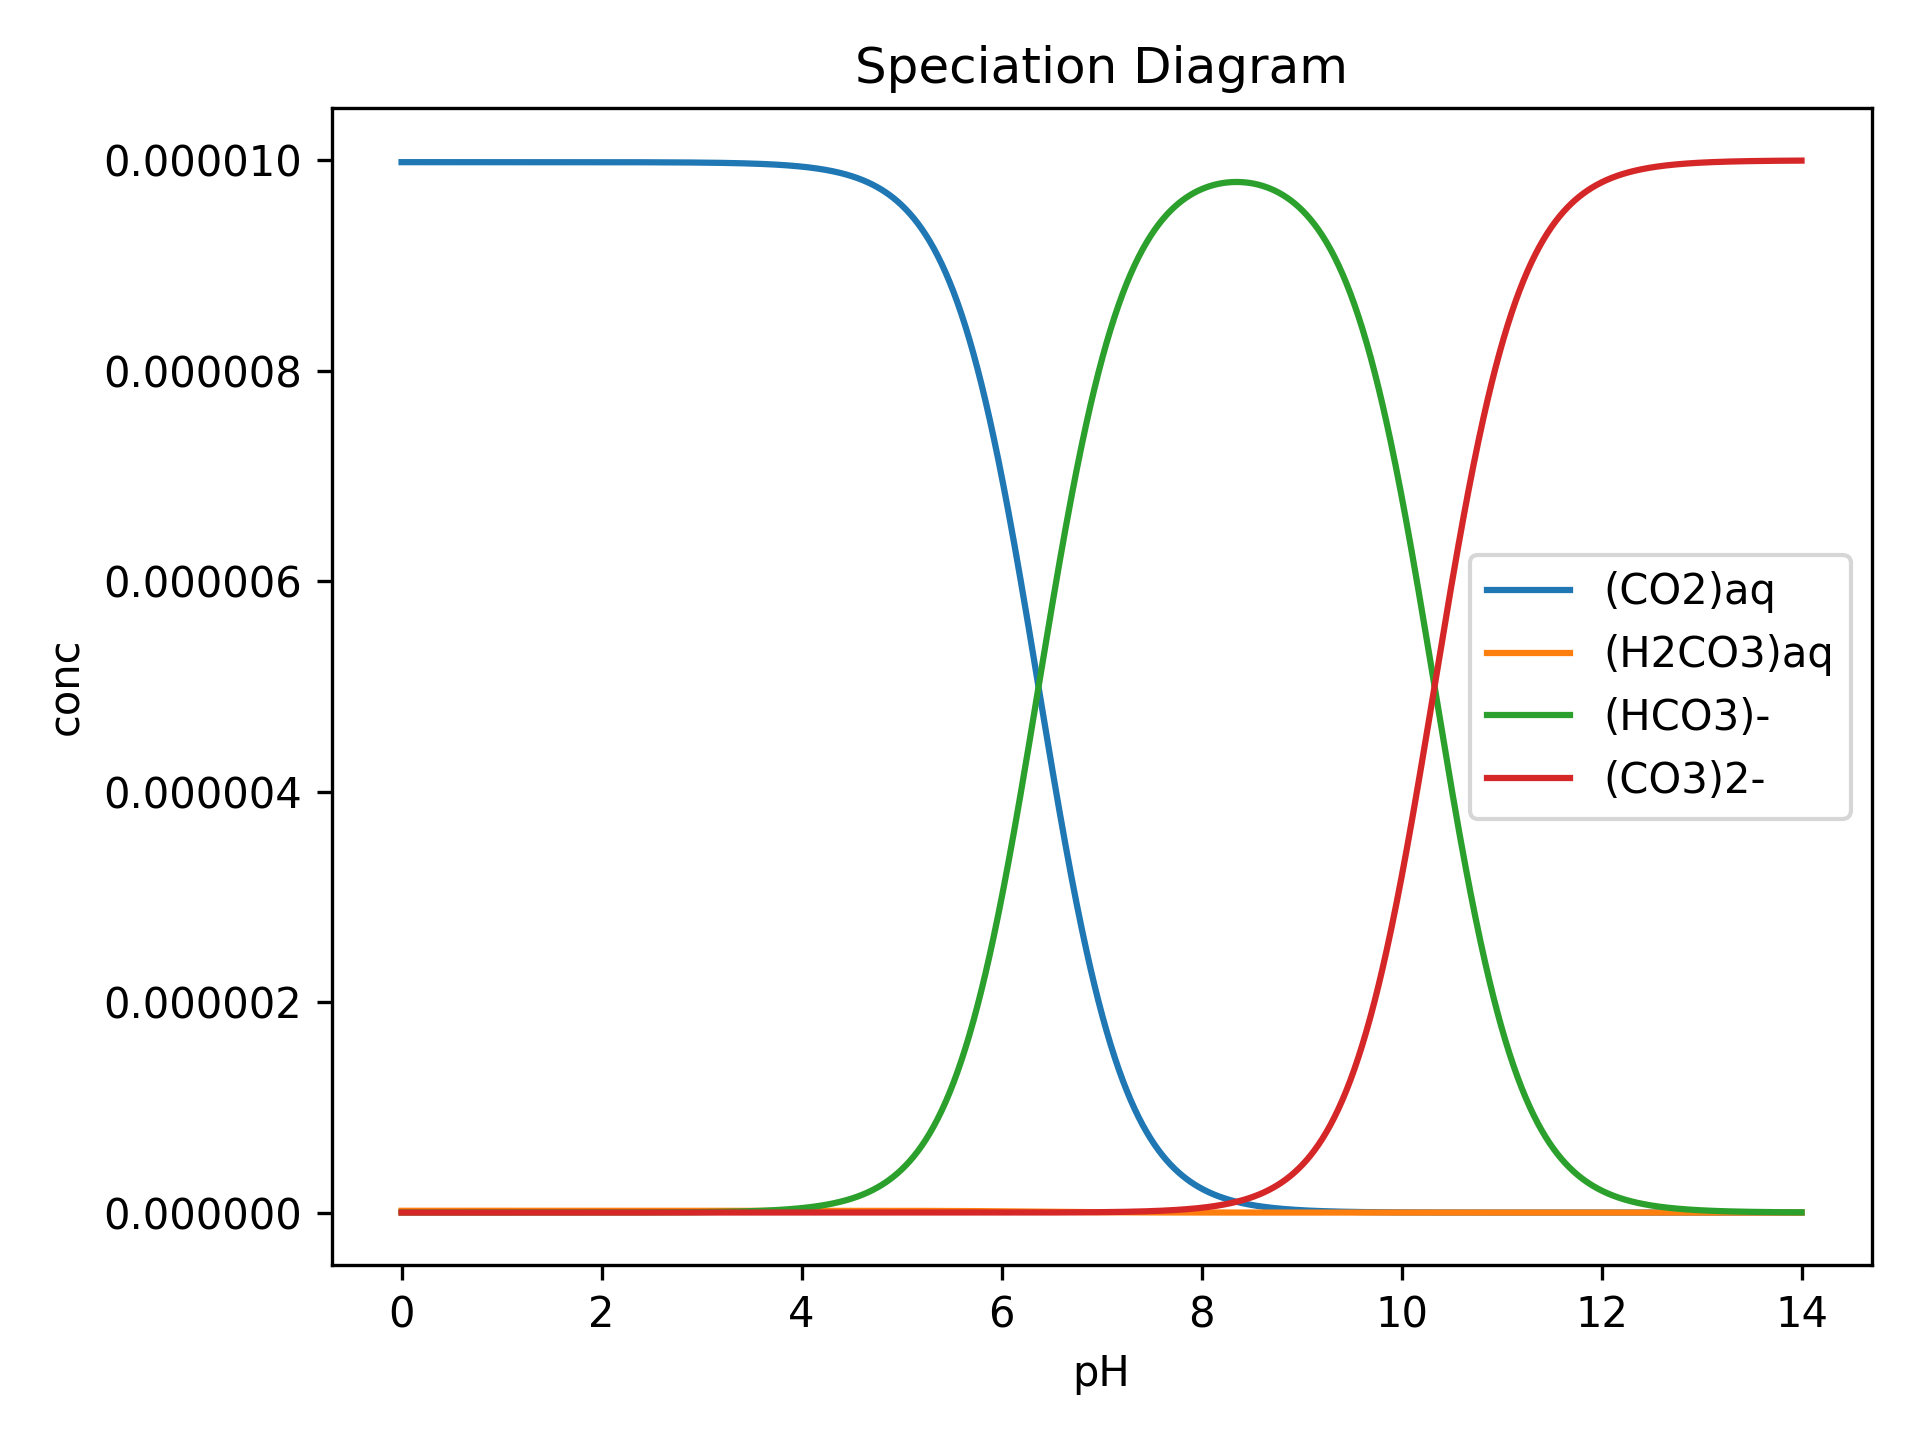
\includegraphics[width=0.7\textwidth]{co2_syst}
					
\item[How test will be performed:] Automated integration test\\
\end{description}
\end{addmargin}


\newpage
\noindent {\bf T\refstepcounter{testnum}\thetestnum \label{T_Comp}: Comparison of 
generated speciation diagram to original}\\
\begin{addmargin}[2em]{0em}
\begin{description}
\item[Type:] Functional, Manual
					
\item[How test will be performed:] This test will compare the diagram generated 
by \progname{} for the FeOH$_3$ system with the diagram generated by Dr. Smith's
MATLAB implementation.  The diagram will be generated in \progname{} by the following
inputs:

\begin{python}
feSys = ChemSys()
feSys.registerRxn(
  "(Fe)3+ + (H2O)l = (Fe(OH))2+ + (H)+ , -2.19"
)
feSys.registerRxn(
  "(Fe)3+ + 2(H2O)l = (Fe(OH)2)+ + 2(H)+ , -5.67"
)
feSys.registerRxn(
  "(Fe)3+ + 4(H2O)l = (Fe(OH)4)- + 4(H)+ , -21.6"
)
feSys.registerTotal(
  "Fe", 0.000010
)
feSys.specGen("fe")
\end{python}

The diagram should be the same as the following:

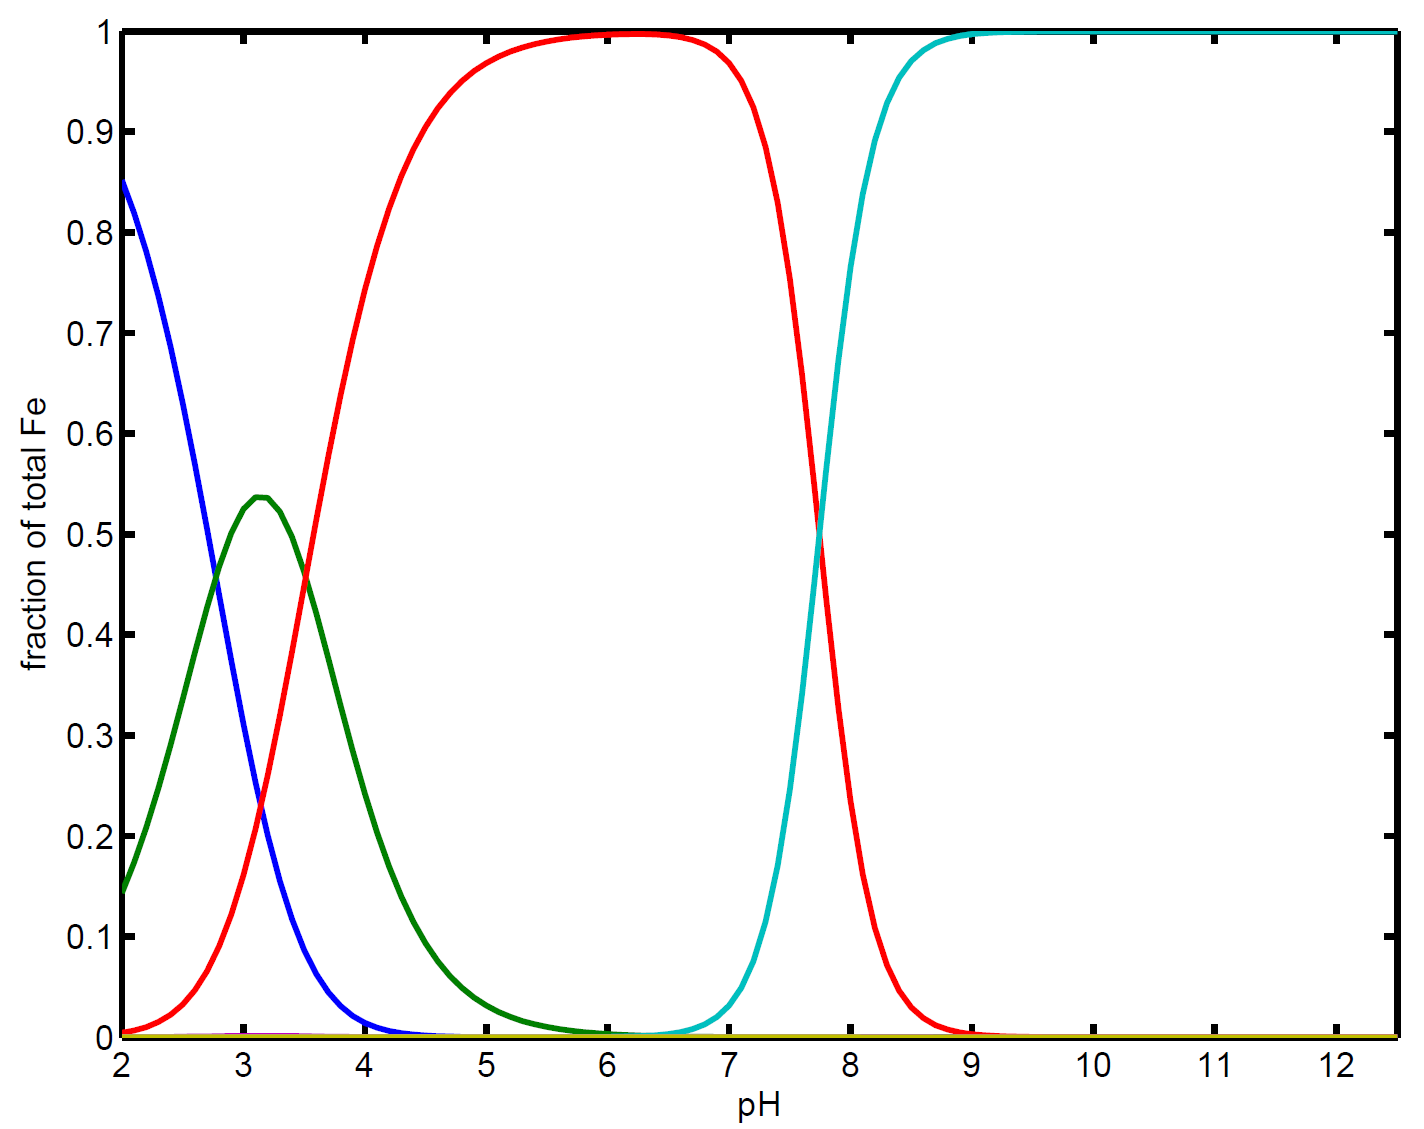
\includegraphics[width=0.7\textwidth]{orig_ref}\\
\end{description}
\end{addmargin}



\subsection{Tests for Nonfunctional Requirements}

		
\noindent {\bf T\refstepcounter{testnum}\thetestnum \label{T_NF_Read}: Readability of 
generated speciation diagram}\\
\begin{addmargin}[2em]{0em}
\begin{description}
\item[Type:] Nonfunctional, Manual
					
\item[How test will be performed:] This is a qualitative test to ensure that the 
diagrams generated by \progname{} are readable (axis labels visible, curves 
distinguishable from each other, \wss{proof read} legend/labelling of curves, etc.).\\
\end{description}
\end{addmargin}


\wss{It wouldn't be bad to add an acceptance test where you explicitly
  plan to ask Dr.\ Smith to review the program.  This would implicitly
  capture functional and nonfunctional requirements, to some extent.}
\spc{I didn't get around to this one :-( }

\section{Traceability Between System Tests and Requirements}
A trace between system tests and requirements is provided in 
\hyperref[tab:reqtrace]{Table~\ref*{tab:reqtrace}}.

\begin{table}[h]
\caption{Requirements Traceability} \label{tab:reqtrace}
\centering
\begin{tabularx}{0.55\textwidth}{p{4cm}X}
\toprule {\bf Requirement} & {\bf Test(s)}\\
\midrule
R1	&	\testref{T_DiagFe}, \testref{T_DiagCO2}, \testref{T_Comp}\\
R2	&	\testref{T_DiagFe}, \testref{T_DiagCO2}, \testref{T_Comp}\\
R3	&	\testref{T_DiagFe}, \testref{T_DiagCO2}, \testref{T_Comp}\\
R4	&	\testref{T_DiagFe}, \testref{T_DiagCO2}, \testref{T_Comp}\\
R5	&	\testref{T_DiagFe}, \testref{T_DiagCO2}, \testref{T_Comp}\\
NF1 & \testref{T_NF_Read}\\
\bottomrule
\end{tabularx}
\end{table}

\newpage		
\section{Unit Testing Plan}
%% NEW

%%%%%%%%%%% PLOTTING MODULE TESTING %%%%%%%%%%%
\subsection{Plotting Module Testing}
\begin{addmargin}[2em]{0em}

\noindent {\bf T\refstepcounter{testnum}\thetestnum \label{T_Plot}: Plotting Test}\\
\begin{addmargin}[2em]{0em}
\begin{description}
\item[Type:] Automatic, Unit
					
\item[Initial State:] N/A
					
\item[Input:] ~\newline

\begin{python}
genDiagram( "test_plot", 
            range(0, 11), 
            "x", 
            [range(0, 11)], 
            "y", 
            ["y1"] )
\end{python}
					
\item[Output:] ~\newline

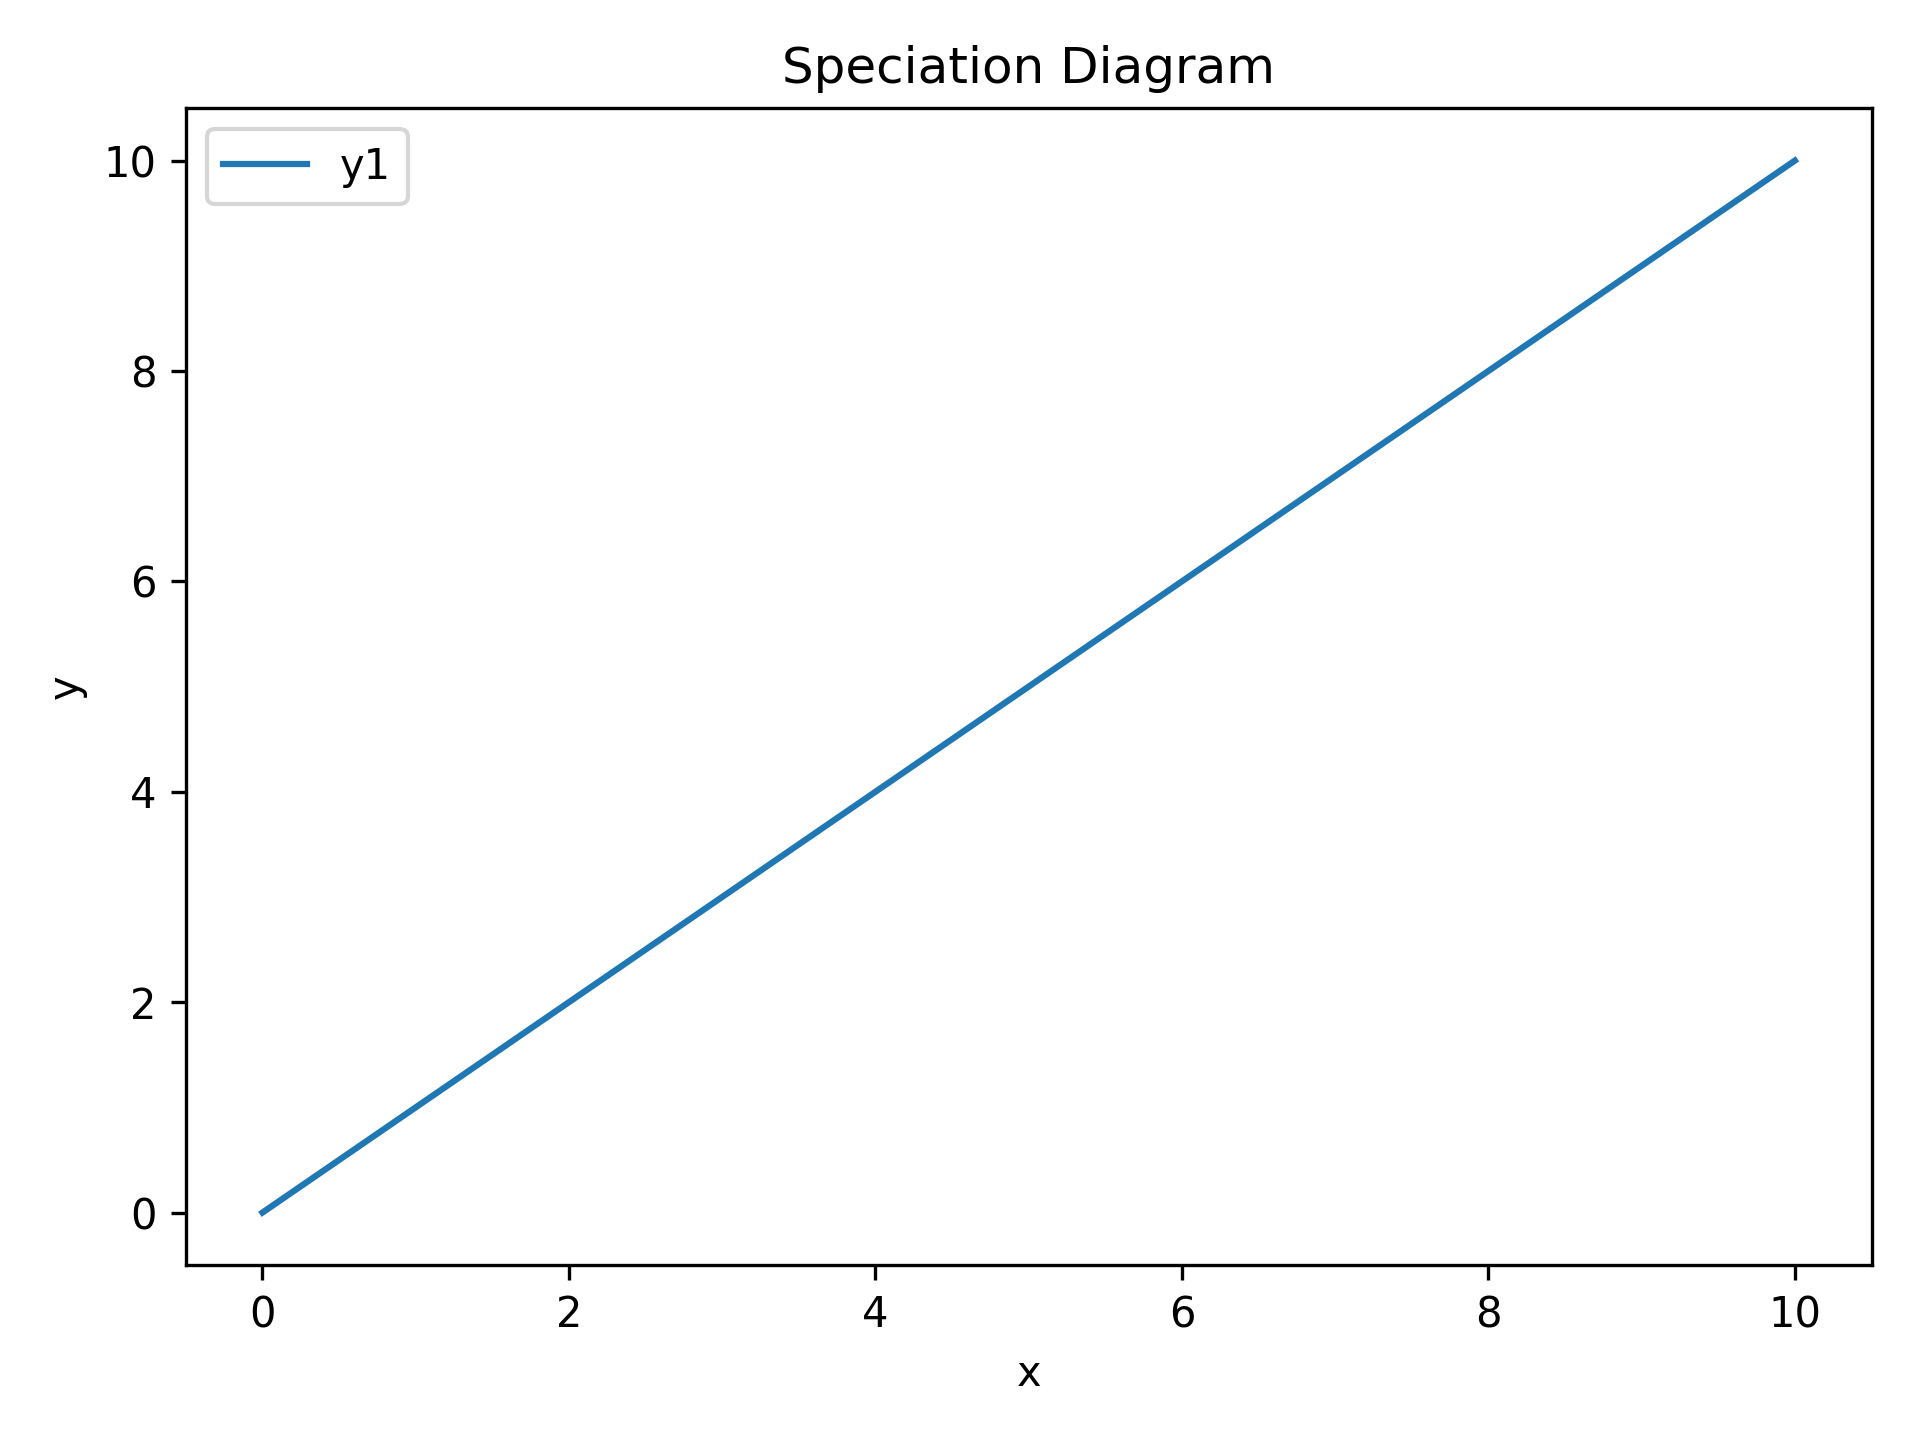
\includegraphics[width=0.7\textwidth]{test_plot_ref}
					
\item[How test will be performed:] Automated unit test\\
\end{description}
\end{addmargin}

\end{addmargin}


%%%%%%%%%%% INPUT CONVERSION MODULE TESTING %%%%%%%%%%%
\subsection{Input Conversion Module Testing}
\begin{addmargin}[2em]{0em}
%%%%

\noindent {\bf T\refstepcounter{testnum}\thetestnum \label{T_ConvFe}: Input conversion of FeOH$_3$ system}\\
\begin{addmargin}[2em]{0em}
\begin{description}
\item[Type:] Automatic, Unit
					
\item[Initial State:] ~\newline

\begin{python}
feSys = ChemSys()
feSys.registerRxn(
  "(Fe)3+ + (H2O)l = (Fe(OH))2+ + (H)+ , -2.19"
)
feSys.registerRxn(
  "(Fe)3+ + 2(H2O)l = (Fe(OH)2)+ + 2(H)+ , -5.67"
)
feSys.registerRxn(
  "(Fe)3+ + 4(H2O)l = (Fe(OH)4)- + 4(H)+ , -21.6"
)
feSys.registerTotal(
  "Fe", 0.000010
)
(fn, _) = makeRootFunc(feSys)

def expectedFe(p, *arg):
  (h, oh) = arg
  (x1, x2, x3, x4) = p
  return ( x2 + h - x1 + 2.19, 
           x3 + 2*h - x1 + 5.67,
           x4 + 4*h - x1 + 21.6,
           log10(10**x1 + 10**x2 + 10**x3 + 10**x4) 
             - log10(0.000010) )
\end{python}
					
\item[Input:] ~\newline

\begin{python}
fn((a, b, c, d), e, f)
\end{python}

For $a$, $b$, $c$, $d$, $e$, $f$ in range -14 to 0.
					
\item[Output:] ~\newline

\begin{python}
expectedFe((a, b, c, d), e, f)
\end{python}

For same values of $a$, $b$, $c$, $d$, $e$, $f$.
					
\item[How test will be performed:] Automated unit test\\
\end{description}
\end{addmargin}


%%%%

\noindent {\bf T\refstepcounter{testnum}\thetestnum \label{T_ConvCO2}: Input conversion of CO$_2$ system}\\
\begin{addmargin}[2em]{0em}
\begin{description}
\item[Type:] Automatic, Unit
					
\item[Initial State:] ~\newline

\begin{python}
co2Sys = ChemSys()
co2Sys.registerRxn(
  "(CO2)aq + (H2O)l = (H2CO3)aq , -2.77"
)
co2Sys.registerRxn(
  "(H2CO3)aq = (HCO3)- + (H)+ , -3.6"
)
co2Sys.registerRxn(
  "(HCO3)- = (CO3)2- + (H)+ , -10.33"
)
co2Sys.registerTotal(
  "C", 0.000010
)
(fn, _) = makeRootFunc(co2Sys)

def expectedCO2(p, *arg):
  (h, oh) = arg
  (x1, x2, x3, x4) = p
  return ( x2 - x1 + 2.77, 
           x3 + h - x2 + 3.6,
           x4 + h - x3 + 10.33,
           log10(10**x1 + 10**x2 + 10**x3 + 10**x4) 
             - log10(0.000010) )
\end{python}
					
\item[Input:] ~\newline

\begin{python}
fn((a, b, c, d), e, f)
\end{python}

For $a$, $b$, $c$, $d$, $e$, $f$ in range -14 to 0.
					
\item[Output:] ~\newline

\begin{python}
expectedCO2((a, b, c, d), e, f)
\end{python}

For same values of $a$, $b$, $c$, $d$, $e$, $f$.
					
\item[How test will be performed:] Automated unit test\\
\end{description}
\end{addmargin}


%%%

\noindent {\bf T\refstepcounter{testnum}\thetestnum \label{T_ConvExc}: Input conversion of empty system}\\
\begin{addmargin}[2em]{0em}
\begin{description}
\item[Type:] Automatic, Unit
					
\item[Initial State:] ~\newline

\begin{python}
emptySys = ChemSys()
\end{python}
					
\item[Input:] ~\newline

\begin{python}
makeRootFunc(emptySys) 
\end{python}
					
\item[Output:] Runtime Error
					
\item[How test will be performed:] Automated unit test\\
\end{description}
\end{addmargin}

\end{addmargin}

%%%%%%%%%%% CALCULATION MODULE TESTING %%%%%%%%%%%
\subsection{Calculation Module Testing}
\begin{addmargin}[2em]{0em}

%%%%


\noindent {\bf T\refstepcounter{testnum}\thetestnum \label{T_CalcExc}: Calculation of empty system}\\
\begin{addmargin}[2em]{0em}
\begin{description}
\item[Type:] Automatic, Unit
					
\item[Initial State:] ~\newline

\begin{python}
emptySys = ChemSys()
\end{python}
					
\item[Input:] ~\newline

\begin{python}
calcSpec(emptySys) 
\end{python}
					
\item[Output:] Runtime Error
					
\item[How test will be performed:] Automated unit test\\
\end{description}
\end{addmargin}

%%%%
\newpage
\noindent {\bf T\refstepcounter{testnum}\thetestnum \label{T_CalcLine}: Calculation of simple system}\\
\begin{addmargin}[2em]{0em}
\begin{description}
\item[Type:] Automatic, Unit
					
\item[Initial State:] ~\newline

\begin{python}
cs = ChemSys()
cs.registerRxn("(T)aq = (H)+ , 0")
\end{python}
					
\item[Input:] ~\newline

\begin{python}
(_, out, _) = calcSpec(cs)
out
\end{python}
					
\item[Output:] ~\newline

\begin{python}
[[10**(-x/100) for x in range(0, 1401)]]	
\end{python}
				
\item[How test will be performed:] Automated unit test\\
\end{description}
\end{addmargin}

\end{addmargin}

%%%%%%%%%%% CALCULATION MODULE TESTING %%%%%%%%%%%
\subsection{Chemical System Module Testing}
\begin{addmargin}[2em]{0em}

%%%%


\noindent {\bf T\refstepcounter{testnum}\thetestnum \label{T_SysBad1}: Register reaction as empty string}\\
\begin{addmargin}[2em]{0em}
\begin{description}
\item[Type:] Automatic, Unit
					
\item[Initial State:] ~\newline

\begin{python}
cs = ChemSys()
\end{python}
					
\item[Input:] ~\newline

\begin{python}
cs.registerRxn("") 
\end{python}
					
\item[Output:] Value Error
					
\item[How test will be performed:] Automated unit test\\
\end{description}
\end{addmargin}

%%%%
\newpage
\noindent {\bf T\refstepcounter{testnum}\thetestnum \label{T_SysBad2}: Register reaction without equilibrium constant}\\
\begin{addmargin}[2em]{0em}
\begin{description}
\item[Type:] Automatic, Unit
					
\item[Initial State:] ~\newline

\begin{python}
cs = ChemSys()
\end{python}
					
\item[Input:] ~\newline

\begin{python}
cs.registerRxn("(H)+") 
\end{python}
					
\item[Output:] Value Error
					
\item[How test will be performed:] Automated unit test\\
\end{description}
\end{addmargin}

%%%%

\noindent {\bf T\refstepcounter{testnum}\thetestnum \label{T_SysBad3}: Register reaction without products}\\
\begin{addmargin}[2em]{0em}
\begin{description}
\item[Type:] Automatic, Unit
					
\item[Initial State:] ~\newline

\begin{python}
cs = ChemSys()
\end{python}
					
\item[Input:] ~\newline

\begin{python}
cs.registerRxn("(H)+ , 0") 
\end{python}
					
\item[Output:] Value Error
					
\item[How test will be performed:] Automated unit test\\
\end{description}
\end{addmargin}

%%%%

\noindent {\bf T\refstepcounter{testnum}\thetestnum \label{T_SysBad4}: Register reaction with bad state}\\
\begin{addmargin}[2em]{0em}
\begin{description}
\item[Type:] Automatic, Unit
					
\item[Initial State:] ~\newline

\begin{python}
cs = ChemSys()
\end{python}
\newpage					
\item[Input:] ~\newline

\begin{python}
cs.registerRxn("(H)bad = (H)bad , 0") 
\end{python}
					
\item[Output:] Runtime Error
					
\item[How test will be performed:] Automated unit test\\
\end{description}
\end{addmargin}

%%%%

\noindent {\bf T\refstepcounter{testnum}\thetestnum \label{T_SysBad5}: Register reaction with bad formula (non-letter symbol)}\\
\begin{addmargin}[2em]{0em}
\begin{description}
\item[Type:] Automatic, Unit
					
\item[Initial State:] ~\newline

\begin{python}
cs = ChemSys()
\end{python}
					
\item[Input:] ~\newline

\begin{python}
cs.registerRxn("(H)bad = (H)bad , 0") 
\end{python}
					
\item[Output:] Runtime Error
					
\item[How test will be performed:] Automated unit test\\
\end{description}
\end{addmargin}

%%%%

\noindent {\bf T\refstepcounter{testnum}\thetestnum \label{T_SysBad6}: Register reaction with bad formula (beginning with lower case)}\\
\begin{addmargin}[2em]{0em}
\begin{description}
\item[Type:] Automatic, Unit
					
\item[Initial State:] ~\newline

\begin{python}
cs = ChemSys()
\end{python}
					
\item[Input:] ~\newline

\begin{python}
cs.registerRxn("(h)+ = (h)+ , 0") 
\end{python}
					
\item[Output:] Runtime Error
					
\item[How test will be performed:] Automated unit test\\
\end{description}
\end{addmargin}

%%%%
\newpage
\noindent {\bf T\refstepcounter{testnum}\thetestnum \label{T_SysBad7}: Register reaction with bad formula (no parentheses)}\\
\begin{addmargin}[2em]{0em}
\begin{description}
\item[Type:] Automatic, Unit
					
\item[Initial State:] ~\newline

\begin{python}
cs = ChemSys()
\end{python}
					
\item[Input:] ~\newline

\begin{python}
cs.registerRxn("H+ = H+ , 0") 
\end{python}
					
\item[Output:] Runtime Error
					
\item[How test will be performed:] Automated unit test\\
\end{description}
\end{addmargin}

%%%%

\noindent {\bf T\refstepcounter{testnum}\thetestnum \label{T_SysBad8}: Register reaction with bad formula (unbalanced parentheses)}\\
\begin{addmargin}[2em]{0em}
\begin{description}
\item[Type:] Automatic, Unit
					
\item[Initial State:] ~\newline

\begin{python}
cs = ChemSys()
\end{python}
					
\item[Input:] ~\newline

\begin{python}
cs.registerRxn("((H)+ = (H)+ , 0") 
\end{python}
					
\item[Output:] Runtime Error
					
\item[How test will be performed:] Automated unit test\\
\end{description}
\end{addmargin}

%%%%

\noindent {\bf T\refstepcounter{testnum}\thetestnum \label{T_SysParen1}: Register reaction with superfluous parentheses}\\
\begin{addmargin}[2em]{0em}
\begin{description}
\item[Type:] Automatic, Unit
					
\item[Initial State:] ~\newline

\begin{python}
cs = ChemSys()
\end{python}
\newpage					
\item[Input:] ~\newline

\begin{python}
cs.registerRxn("((H))+ = (H)+ , 0") 
\end{python}
					
\item[Output:] No Error
					
\item[How test will be performed:] Automated unit test\\
\end{description}
\end{addmargin}

%%%%

\noindent {\bf T\refstepcounter{testnum}\thetestnum \label{T_SysParen2}: Register reaction with high parenthesis nesting}\\
\begin{addmargin}[2em]{0em}
\begin{description}
\item[Type:] Automatic, Unit
					
\item[Initial State:] ~\newline

\begin{python}
cs = ChemSys()
\end{python}
					
\item[Input:] ~\newline

\begin{python}
cs.registerRxn("((H(OH)2(H)))l = (H)+ , 0") 
\end{python}
					
\item[Output:] No Error
					
\item[How test will be performed:] Automated unit test\\
\end{description}
\end{addmargin}

%%%%

\noindent {\bf T\refstepcounter{testnum}\thetestnum \label{T_TotNeg}: Register negative element total}\\
\begin{addmargin}[2em]{0em}
\begin{description}
\item[Type:] Automatic, Unit
					
\item[Initial State:] ~\newline

\begin{python}
cs = ChemSys()
\end{python}
					
\item[Input:] ~\newline

\begin{python}
cs.registerTotal("H", -1) 
\end{python}
					
\item[Output:] Runtime Error
					
\item[How test will be performed:] Automated unit test\\
\end{description}
\end{addmargin}

%%%%
\newpage
\noindent {\bf T\refstepcounter{testnum}\thetestnum \label{T_TotZero}: Register zero element total}\\
\begin{addmargin}[2em]{0em}
\begin{description}
\item[Type:] Automatic, Unit
					
\item[Initial State:] ~\newline

\begin{python}
cs = ChemSys()
\end{python}
					
\item[Input:] ~\newline

\begin{python}
cs.registerTotal("H", 0) 
\end{python}
					
\item[Output:] Runtime Error
					
\item[How test will be performed:] Automated unit test\\
\end{description}
\end{addmargin}

%%%%

\noindent {\bf T\refstepcounter{testnum}\thetestnum \label{T_TotPos}: Register positive element total}\\
\begin{addmargin}[2em]{0em}
\begin{description}
\item[Type:] Automatic, Unit
					
\item[Initial State:] ~\newline

\begin{python}
cs = ChemSys()
\end{python}
					
\item[Input:] ~\newline

\begin{python}
cs.registerTotal("H", 1) 
\end{python}
					
\item[Output:] No Error
					
\item[How test will be performed:] Automated unit test\\
\end{description}
\end{addmargin}

%%%%

\end{addmargin}

%%% END NEW

\newpage
\section{Traceability Between Unit Tests and Modules}
A trace between unit tests and modules is provided in 
\hyperref[tab:modtrace]{Table~\ref*{tab:modtrace}}.

\begin{table}[h]
\caption{Module Traceability} \label{tab:modtrace}
\centering
\begin{tabularx}{0.90\textwidth}{lX}
\toprule {\bf Module} & {\bf Test(s)}\\
\midrule
M1 & implemented by OS; no tests required\\
M2 & external interface; no explicit testing; covered implicitly\\
M3 & \testref{T_SysBad1}, \testref{T_SysBad2}, \testref{T_SysBad3}, 
\testref{T_SysBad4}, \testref{T_SysBad5}, \testref{T_SysBad6}, 
\testref{T_SysBad7}, \testref{T_SysBad8}, \testref{T_SysParen1},
\testref{T_SysParen2}, \testref{T_TotNeg}, \testref{T_TotZero},
\testref{T_TotPos} \\
M4 & data structure; no explicit testing; covered implicitly\\
M5 & data structure; no explicit testing; covered implicitly\\
M6 & \testref{T_ConvFe}, \testref{T_ConvCO2}, \testref{T_ConvExc}\\
M7 & \testref{T_CalcExc}, \testref{T_CalcLine}\\
M8 & implemented by Python; no tests required\\
M9 & \testref{T_Plot}\\
\bottomrule
\end{tabularx}
\end{table}

%\bibliographystyle{plainnat}

%\bibliography {../../ReferenceMaterial/References}

\end{document}